\documentclass{article}
\usepackage[utf8]{inputenc}
\usepackage[T1]{fontenc}
\usepackage{graphicx}
\usepackage{hyperref}
\usepackage{geometry}
\geometry{margin=1in}

\title{ATELLA}
\date{Encyclopaedia Britannica (1771)}

\begin{document}
\maketitle

\section*{Historical source}
\textbf{Entry ID:} \texttt{entry-atella-2171} \\
\textbf{Volume ID:} 144850373 \\
\textbf{Character Count:} 720

\subsection*{Extracted Text}
ATELLA, an ancient town of Gargania in Italy, between Capua and Nespolis. From this town the \_Atlana fabule, or Atelani Inda\_, took their name. There were alto called \_Ofis\_, from their invasion, in whole territory Ashala by. They were generally a species of force, interlarded with much ribalry and buffoonery and foundoreste were ecordix or intestinalis preferred between the each of other plays. The authors thank these forces were not reckoned among the common players, nor deemed infamous , but retained the rights of their tribe, and might be listed for folders, the privilege only of free men. The ruins of this town are full to be feen about 11 miles from the modern Averfa, which was built out of its materials.



\section*{Source record}
\begin{itemize}
\item \textbf{Dataset:} \texttt{NationalLibraryOfScotland/encyclopaedia\_britannica\_illustrated}
\item \textbf{Dataset Revision:} \texttt{309f765b1ecc83e0a7f7762e44b4a927a7555443}
\item \textbf{Page ID:} \texttt{britannica:309f765b1ecc83e0a7f7762e44b4a927a7555443:train:2171} \\
  \textbf{Filename:} \texttt{page-2171-f8869fa95f19.jpg} \\
  \textbf{Row Index:} 2171 \\
  \textbf{SHA256:} \texttt{f8869fa95f190d0e...}
\end{itemize}

\begin{figure}[h]
\centering
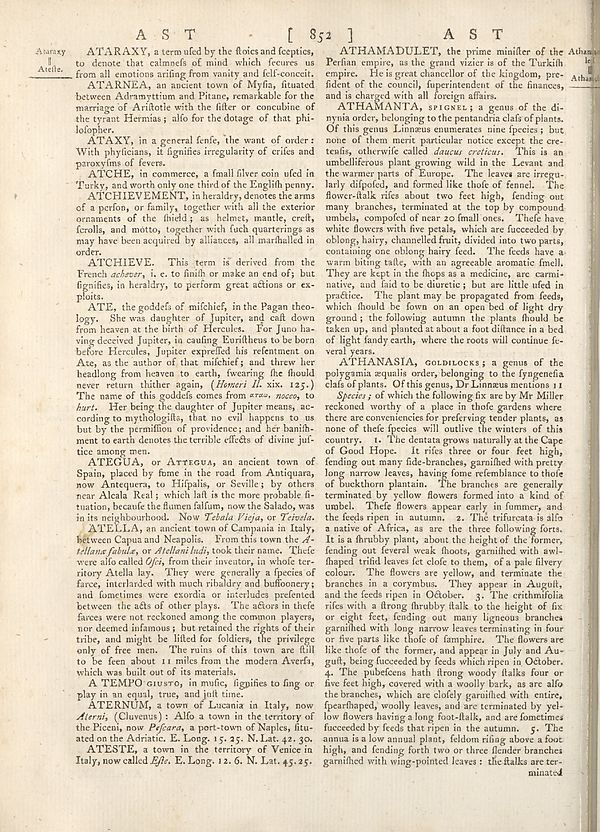
\includegraphics[width=0.85\textwidth]{../scans/page-2171-f8869fa95f19.jpg}
\caption*{Source scan: \texttt{page-2171-f8869fa95f19.jpg}}
\end{figure}

\end{document}
